\documentclass{article}
\usepackage{graphicx,mathtools,amsmath,amssymb, dirtytalk} % Required for inserting images

\setlength{\oddsidemargin}{0in}
\setlength{\textwidth}{6.5in}
\setlength{\topmargin}{-.55in}
\setlength{\textheight}{9in}
\pagestyle{empty}


\title{Scientific Computation II HW4}
\author{Michael Nameika}
\date{May 2023}

\begin{document}

\maketitle

\section*{Exercise 1: Application of RBF Interpolation - 2D reconstruction from a point cloud}
Consider an implicit (closed) curve in 2D
\[f(x,y) = 0\]
given by a parameterization $x = x(t)$, $y = y(t)$, $t \in [0,L]$. For a choice of parameter values $\{t_j\} = \{t_1,\dots, t_N\}$, consider the \say{point cloud} $\{\mathbf{x}_j = (x_j, y_j) = (x(t_j), y(t_j))\}$. The goal of this exercise is to reconstruct (approximately) the implicity function from the given point cloud.
\begin{itemize}
    \item[\textbf{Step 1}:] Find an (outer) normal direction $\mathbf{n}_j$ to the curve at each point $\mathbf{x}_j$.
    \newline\newline

    
    \item[\textbf{Step 2}:] Fix $\alpha > 0$ small and consider the inner and outer points
    \[\mathbf{x_j}^- = \mathbf{x}_j - a\mathbf{n}_j, \hspace{0.75em} \mathbf{x}_j^+ = \mathbf{x}_j + \alpha \mathbf{n}_j.\]

    \item[\textbf{Step 3}:] Interpolate the $3N$ data $(\mathbf{x}_j^-, -\alpha)$, $(\mathbf{x}_j, 0)$, $(\mathbf{x}_j^+, \alpha)$ using RBF interpolants, that is, find a function $F: \mathbb{R}^2 \to \mathbb{R}$, 
    \[F(\mathbf{x}) = \sum_{j=1}^Nc_j\phi(\|\mathbf{x} - \mathbf{x}_j\|)\]
    such that $F(\mathbf{x}_j) = 0$ and $F(\mathbf{x}_j^-) = -\alpha, F(\mathbf{x}_j^+) = \alpha$.
    \newline\newline

    \item[\textbf{Step 4}:] Restrict $F$ to the level set $F(x,y) = 0$ to obtain the RBF interpolation for the implicit curve $f(x,y) = 0$.
    \newline\newline
\end{itemize}
Implementing the pointcloud RBF interpolation in \verb+MATLAB+, (see attached \verb+myPointCloudRBF.m+ script) we find the following level curves and surfaces for a few select point clouds:
\begin{figure}[h!]
    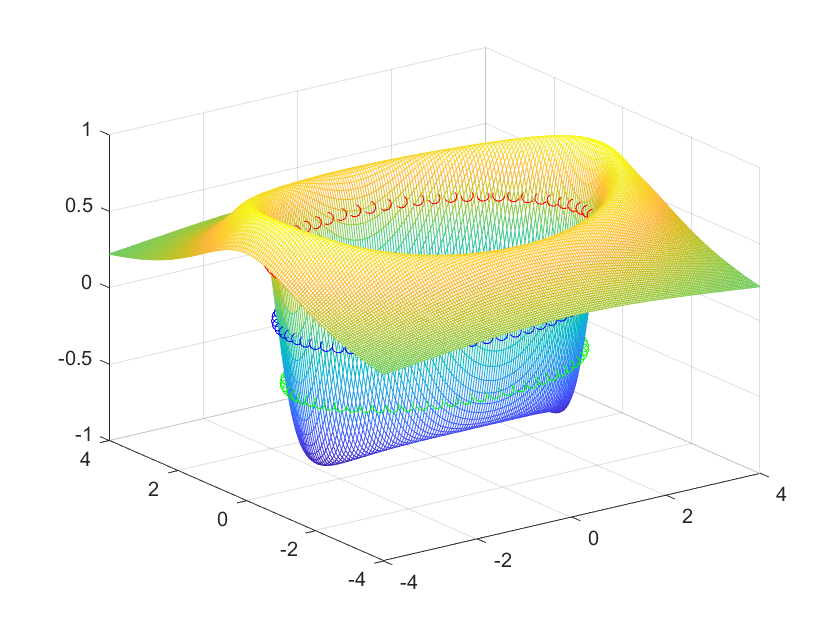
\includegraphics[scale = 0.3]{ellipsePCSurf.png}
    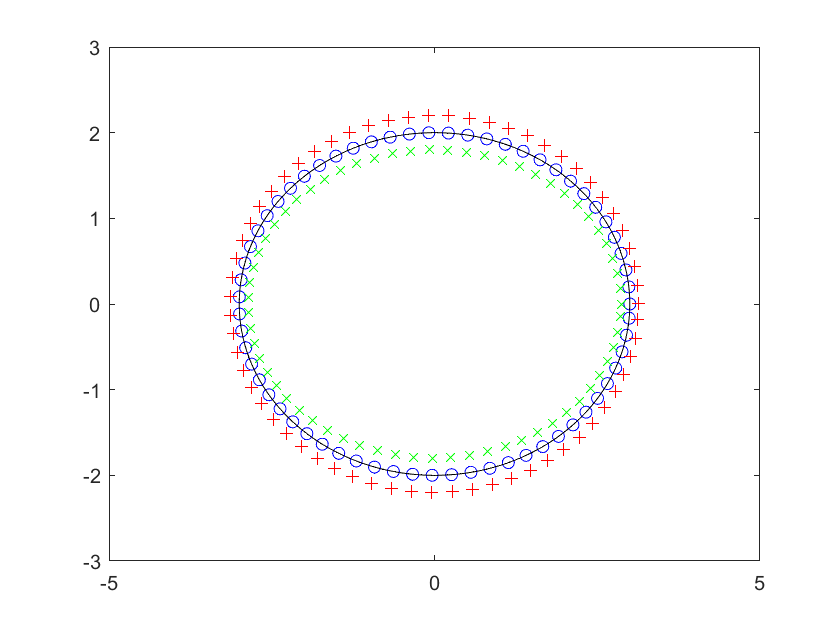
\includegraphics[scale = 0.3]{implicitellipseRBF.png}
    \centering
    \caption{Ellipse Point Cloud with $\alpha = 0.4$, $r_x = 3$, $r_y = 2$ and IMQ RBF interpolant}
\end{figure}
\begin{figure}[h!]
    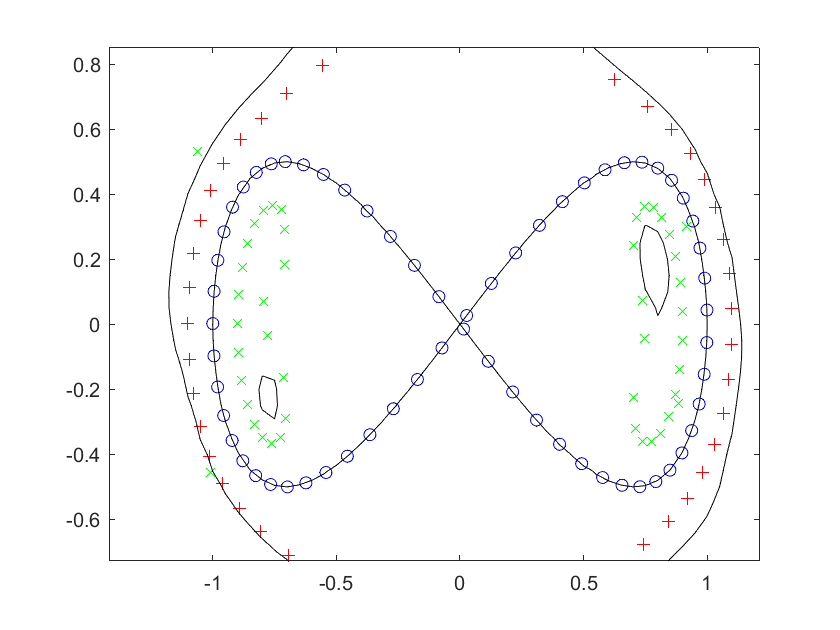
\includegraphics[scale = 0.4]{infinitySymbolCurve.png}
    \centering
    \caption{Infinity Lissajous Curve with $\alpha = 0.1$ and IMQ}
\end{figure}
\begin{figure}[h!]
    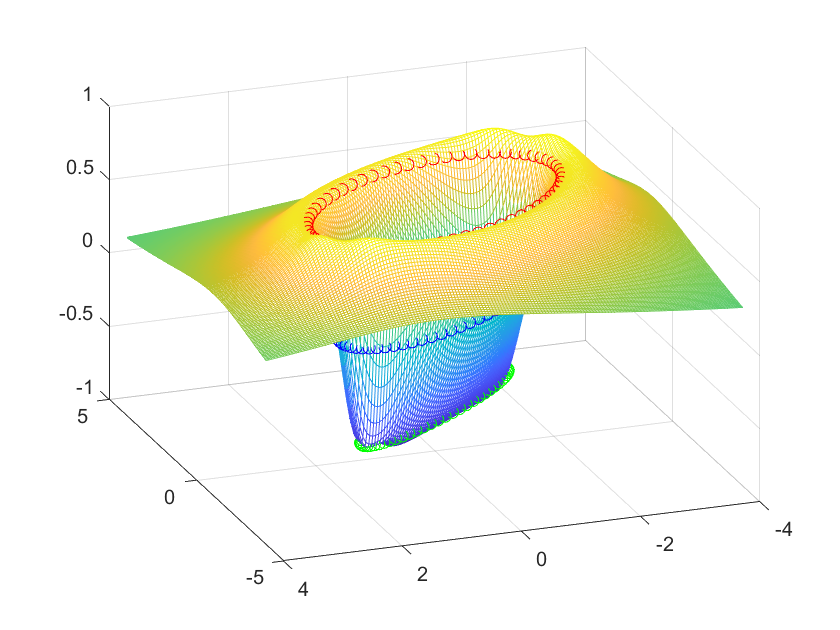
\includegraphics[scale = 0.3]{skewedEllipseSurf.png}
    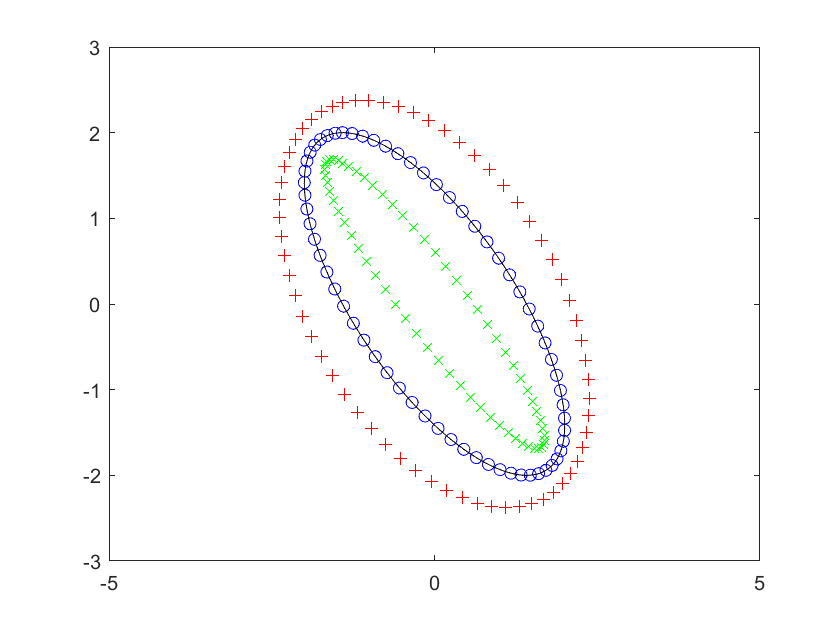
\includegraphics[scale = 0.3]{skewedEllipseCurve.png}
    \centering
    \caption{"Skewed" ellipse with $\alpha = 0.7$ and IMQ}
\end{figure}

\end{document}
